% Author: Nikitha Jayant Bangera
% Version: 1.0

\documentclass[12pt, a4paper]{report}
\usepackage[left=2.5cm, right=2.5cm, top=1cm, bottom=1.5cm]{geometry}
\usepackage[utf8]{inputenc}
\usepackage{amssymb}
\usepackage{amsmath}
\usepackage{latexsym}
\usepackage[normalem]{ulem}
\usepackage{array}
\usepackage{graphicx, tabularx}
\usepackage[backend=biber,
style=numeric,
sorting=none,
isbn=false,
doi=false,
url=false,
]{biblatex}\addbibresource{bibliography.bib}
\usepackage{biblatex}
\usepackage{array,multirow}
\usepackage{longtable}

\date{}

\title{
\includegraphics[width=10cm,height=5cm]{Con_Logo1.jpg}\\\\}
\author{
\LARGE{Eternity: Numbers}
\\\\
A project report presented for the course\\ 
SOEN 6481 \\\textit{Software Requirements Specifications}
\\ \\ 
\\ \Large{Author Name}
\\ Nikitha Jayant Bangera
\\\\ \\
Under the guidance of\\
Professor Pankaj Kamthan
}
%%%%%%%%%%%%%%%%%%%%%%%%%%%%%%%%%%%%%%%%%%%%%%%%%%%%%%%%%%%%%%%%%%%%%%%
\begin{document}
\thispagestyle{headings}
	\maketitle
\pagenumbering{roman}

\thispagestyle{empty}
\chapter*{Acknowledgements}
I would like to express my sincere thanks to Professor Pankaj Kamthan for his advice and encouragement throughout the First deliverable of the Eternity: Numbers project, as well as to my Technical Lab Assistant for his guidance throughout the first phase of the project. 
\thispagestyle{empty}
\begin{abstract}
%\lipsum[1-2]
The document tries to put some light on the understanding of an irrational number, The Champernowne Constant. A brief description of the constant and some of its applications are included in the report. A research and interview on the constant was conducted with a resource who is familiar with Champernowne constant. My interviewee tried to answer most common questions about the constant in a questionnaire that also describes some applications of Champernowne constant. Based on the understanding of Champernowne Constant, a calculator application is to be built, that uses this constant to perform certain operations. This document also gives the basic design details on how the product would look like,what operations is it capable of, its algorithm and use cases.
\end{abstract}

\tableofcontents
\thispagestyle{plain}
\listoffigures
\listoftables

\chapter{Introduction}
\pagenumbering{arabic}
\section{Champernowne's Constant Definition}
\quad Champernowne Constant is a real number whose decimal digits are obtained by concatenating the decimal expansions of the successive positive integers:\\\\
\hspace*{30mm} $C_{10}$ = 0.12345678910111213141516…\\\\
It is named after economist and mathematician David G. Champernowne, who published it as an undergraduate in 1933.\\
\section{Champernowne Constant as an Infinite series}
\quad The Champernowne constants can be expressed exactly as infinite series:\\\\
\hspace*{30mm} $\displaystyle C_m = \sum_{n=1}^{\infty} \frac{n}{{10_b}^{\displaystyle (\sum_{k=1}^n \lceil {log_{10}}_b (k+1) \rceil)}}$\\\\
where $\lceil x \rceil $ = ceiling(x), ${10_b}^x = b^x$ in base 10, ${log_{10}}_b (x) = {log_b}_{10} (x)$ and {\it b} is the base of the constant.\\
\section{Continued Fraction Expansion}
\quad The Continued Fraction Expansion (CFE) of the Champernowne constant turns out to be a set large numbers with various spikes. Kurt Mahler showed that the constant is transcendental; therefore, its continued fraction does not terminate and is aperiodic (because it is not an irreducible quadratic). The terms in the continued fraction expansion exhibit very erratic behaviour, with extremely large terms appearing between many small ones. The CFE begins with 0; 8, 9, 1, 149083, 1, 1, 1, 4, 1, 1, 1, 3, 4, 1, 1, 1, 15, and the coefficient in position 18 has 166 digits. The large number at position 18 has 166 digits, and the next very large number at position 40 of the continued fraction has 2504 digits. The fact that there are such large numbers as terms of the continued fraction expansion is equivalent to saying that the convergents obtained by stopping before these large numbers provide an exceptionally good approximation of the Champernowne constant.\\\\

\begin{figure}
    \centering
    \fbox{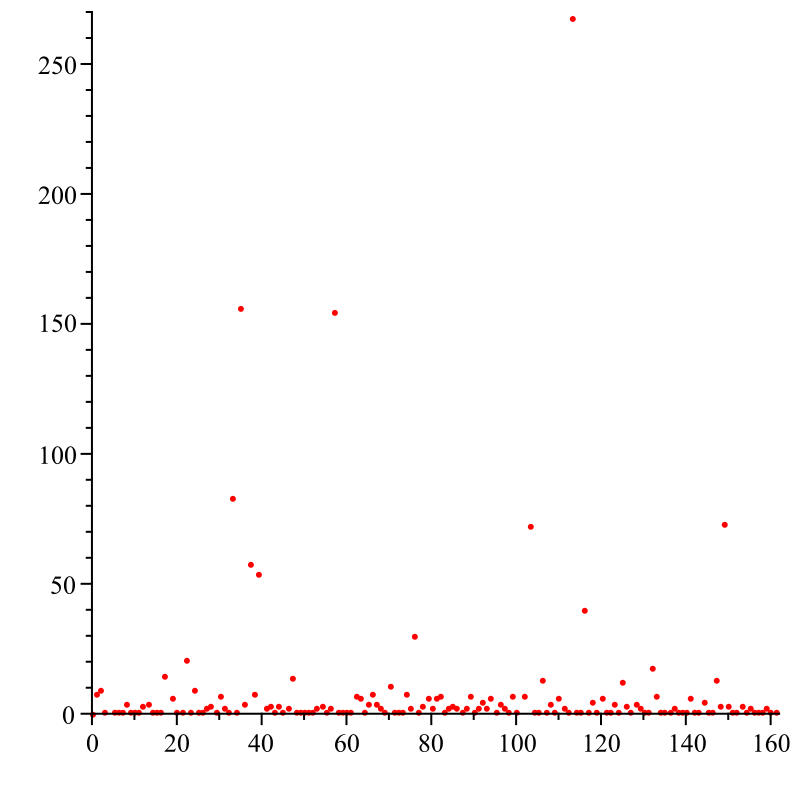
\includegraphics[width=100mm]{Champernowne_Constant.png}}
    \caption{The first 161 quotients of the Champernowne constant.}
    \label{fig:The first 161 quotients of the Champernowne constant.}
\end{figure}

\chapter{Interview}
\label{Chap2}
\section{Brief introduction about the Interviewee}
{\bf Name} : Megha Kamath \\
{\bf Qualification} : Masters in Mathematics \\
{\bf Reason behind opting the interviewee} : My Interviewee is pursuing Masters in Mathematics and it was obvious for me to work with her to better understand about the Champernowne constant and its applications.
\section{Interview Questions on Champernowne Constant}
\begin{enumerate}
	\item Could you mention some areas where Champernowne constant can be applied?
	\\ {\it The Champernowne constant has seemingly random numbers which are clearly well determined. This property could be useful in functional programming contexts where one would need explicit randomness which is entirely deterministic. For example, the C2 (Base 2) value of the Champernowne constant can be used as a binary random number to trigger true or false conditions randomly.}
	\item Could you mention the properties of the Champernowne constant?
	\begin{enumerate}
	{\it \item The constant given by 0.123456789101112 . . . is normal in base ten.
	\item The constant is transcendental.
	\item The constant also has a peculiar continued fraction expansion. It namely contains exceptionally large terms throughout the expansion.}
	\end{enumerate}
	\item Is Champernowne constant a Liouville number?
	\\ {\it No. Champernowne constant and Liouville numbers are both transcendental but Champernowne constant is irrational and Liouville numbers are almost rational and can be approximated quite closely by sequences of rational numbers than any algebraic irrational numbers.}
	\item Is Champernowne constant as useful as  \( \pi \) constant?
	\\ {\it The Champernowne constant is quite useful. But Pi is a constant which is there almost everywhere in mathematics. }
	\item Does it appear in any sort of geometric solutions like  \( \pi \) does?
	\\ {\it The Champernowne constant cannot be represented as a finite number due to which there have been no reported utilization in geometry.}
	\item How often do you use the Champernowne constant?
	\\ {\it As a student of pure mathematics I do not use the Champernowne constant quite often.}
	\item Has the Champernowne constant ever been used in any major proofs? 
	\\ {\it No.}
	\item Can it be expressed in terms of e,  \( \pi \) or both? 
	\\ {\it No.}
	\item What works of Alan Turing and David Champernowne made use of the Champernowne constant?
	\\ {\it Notably, There were two major works of Alan Turing and David Champernowne, the TuroChamp and Round the house Chess. But the Champernowne constant is not mentioned to have been in any of these machines.}
	\item Of all the base versions of Champernowne constants which particular Champernowne sequence has been vastly used?
	\\{\it Base 2 (C\textsubscript{2}) and Base 10 (C\textsubscript{10}).}
	\item Who and How was Champernowne constant proved Transcendental? 
	\\ {\it The Champernowne constant was shown to be transcendental by Kurt Mahler in 1937.}
	\item What are the alternatives available for Champernowne constant?
	\\ {\it None.}
	\item Is Champernowne constant used in Turochamp or Round the house Chess? if Yes, how does it fit into the algorithms of these games?
	\\ {\it No. }
	\item Do you think of any problem where Champernowne Constant would be a perfect fit to be used?
	\\ {\it I can actually think of 2, One being a Random Binary digit generator where Champernowne Constant of Base 2 would be a perfect fit and Two, Given a sequence of numbers (to base 10), How to calculate the position of any random number. I think Champernowne constant fits well into these scenarios. }
\end{enumerate}
\section{Analysis of the Interview}
\quad The Interviewee had moderate knowledge about the Champernowne constant. She was able to explain the basic characteristics of the constant with logical examples (mentioned in the response to the interview questions). The practical applications of the constant have been limited and the interviewee was able to explain one particular area where the constant (its base 2 value) is widely used to generate the randomized binary numbers.

\chapter{User model: Persona Template}
\begin{center}
\begin{tabular}{ | m{40em} | } 
\hline
\\\textbf{Private Information} \\
\begin{minipage}{0.70\textwidth}
\begin{itemize}
    \setlength{\itemsep}{0pt}
    \item Name: Megha Kamath
    \item Qualification: Currently pursuing Masters in Mathematics
    \item University: Mangalore University, Karnataka, India
    \item Megha lives in Karnataka, India with her parents.
    \item She loves to read fictional novels and also cooking is her favourite pass-time.
\end{itemize}
\end{minipage}
\begin{minipage}{0.3\textwidth}
\fbox{
\includegraphics[width=\linewidth, height=4cm]{student.jpg}}
\end{minipage}
\\
\hline
\\\textbf{Use of Number, relation to Number} \\
Based on the conversation with interviewee -\\
\begin{itemize}
    \setlength{\itemsep}{0pt}
    \item The Champernowne constant has seemingly random numbers which are clearly well determined. This property could be useful in functional programming contexts where one would need explicit randomness which is entirely deterministic.
    \item  Base 2 of the Champernowne constant is in functional programming as a Random Binary Digit Generator.
\end{itemize}
\\
\hline
\\\textbf{Description of work or daily life} \\
\begin{itemize}
    \setlength{\itemsep}{0pt}
    \item Megha is in her First Year of Masters in Mathematics. Her specialization is Pure Mathematics.
    \item She has moderate knowledge about the Champernowne Constant.
    \item She does not use the Champernowne constant quite often as her specialization is Pure Mathematics.
\end{itemize}
\\
\hline

\end{tabular}
\begin{tabular}{ | m{40em} | }
\hline
\\\textbf{Other uses or relations to the Number} \\
\begin{itemize}
     \setlength{\itemsep}{0pt}
    \item As per Megha's research, the Champernowne constant was never used in major proofs.
    \item Due to the constant's inefficient nature, the constant is mostly avoided in mathematical calculations.
\end{itemize}
\\
\hline
\\\textbf{Influencers that surround the persona and that may influence choices}\\
\begin{itemize}
    \setlength{\itemsep}{0pt}
    \item Professors
    \item Friends
    \item Classmates
\end{itemize}
\\
\hline
\end{tabular}
\end{center}

\chapter{Problem Domain Model}
\section{UML Class Diagram}
Figure 4.1 shows the Class diagram of the Eternity: Numbers system which behaves as a calculator application that has an option for generating Champernowne Constant.
\begin{figure}[h]
    \centering
    \fbox{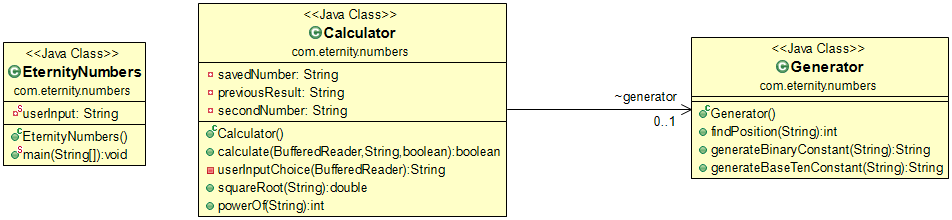
\includegraphics[width=160mm,height=50mm]{EternityNumbersClassDiagram.png}}
    \caption{UML Class Diagram of Eternity: Numbers}
    \label{fig:UML Class Diagram of Eternity: Numbers}
\end{figure}

\begin{itemize}
    \item \textbf{Class: EternityNumbers.java:} Java class that implements the main method to start the application. This class calls the calculate method of the calculator class.
    \item \textbf{Class: Calculator.java:} Is the Java class that performs the following operations:
    \begin{itemize}
        \item Allows user to pick an operation to perform calculations,
        \item Invokes the relevant operational case to process user requests, calls the generator class to perform calculations involving Champernowne Constant and
        \item Display the processed/calculated result to user.
    \end{itemize}
    \item \textbf{Class: Generator.java:} This class performs key operations on Champernowne constant. It has methods to generate Champernowne Constant of Base 10 and Base 2 values and also has a method to find a position of a random number in Base 10 Champernowne Constant.
\end{itemize}

\chapter{Use Case Model}
\section{UML Use Case Diagram}
\quad The following diagram shows the use case view of Eternity Numbers calculator for Champernowne Constant followed by the Activity diagram and sequence diagrams in sections 5.2 and 5.3

\begin{figure}[h]
    \centering
    \fbox{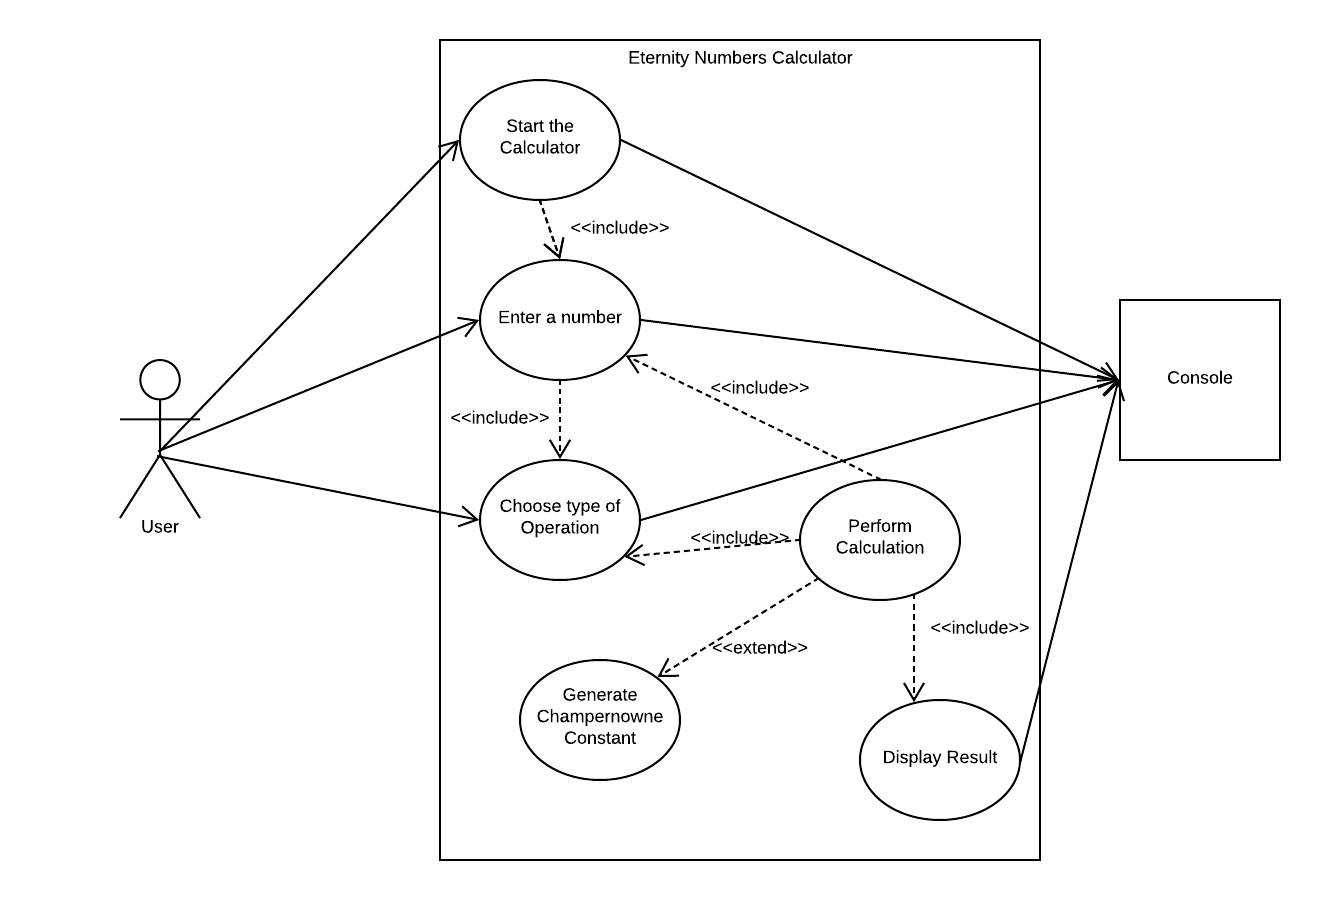
\includegraphics[width=160mm, height=100mm]{ChampernowneUseCase.png}}
    \caption{UML Use Case diagram of Eternity: Numbers}
    \label{fig:UML Use Case diagram of Eternity: Numbers}
\end{figure}

Steps in the Use case model of Eternity numbers calculator (Refer to Figure 5.1):
\begin{enumerate}

    \item User starts the calculator application i.e. Eternity: Numbers calculator. The application displays a set of operations , which a user can pick to perform various operations.
    \item User selects the required operation like addition, subtraction, finding a position of a number in Champernowne Constant, Generating a Champernowne Constant etc.
    \item The applications prompts the user to enter required input values to perform the opetation.
    \item User enters the number.
    \item The system processes user's input and displays results to the user.
\end{enumerate}
\section{UML Activity Diagram}
Figure 5.2 shows the Activity diagram representation of the above use case. If the user selects any other constant other than the Champernowne constant, a relevant message is displayed that the feature is not available as this version of the product focuses on Champernowne Constant only.\\\\
%\hspace{15mm}
\begin{figure}[!h]
    \centering
    \fbox{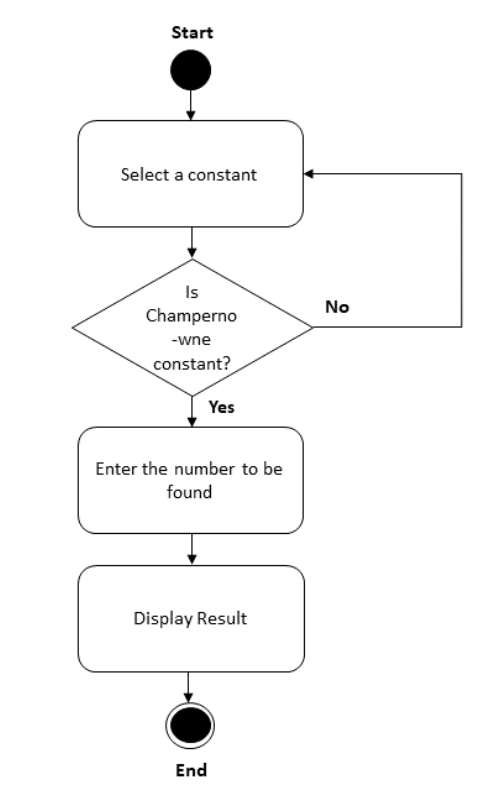
\includegraphics[width=50mm, height=70mm]{ChampernowneActivity.PNG}}
    \caption{UML Activity diagram of Eternity: Numbers}
    \label{fig:UML Activity diagram of Eternity: Numbers}
\end{figure}

\section{Sequence diagram}
Figure 5.3 shows the sequence diagram of the Eternity Numbers caculator application
\begin{figure}[h]
    \centering
    \fbox{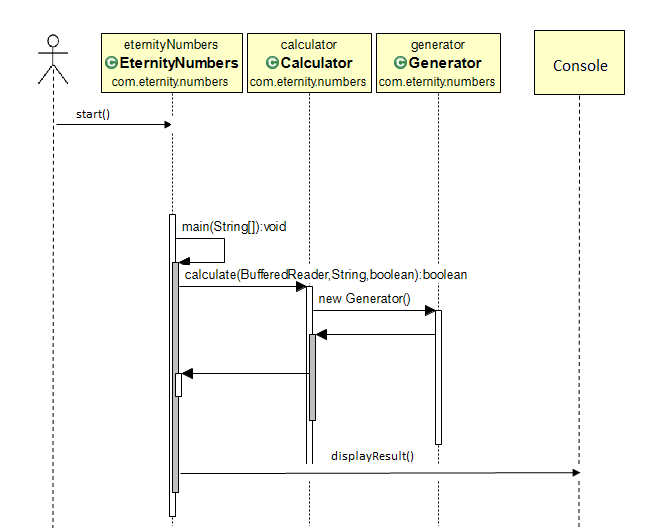
\includegraphics[width=120mm, height=80mm]{EternityNumbersSequenceDiagram.png}}
    \caption{UML Sequence diagram of Eternity: Numbers}
    \label{fig:UML Sequence diagram of Eternity: Numbers}
\end{figure}

\section{Normal Scenario of Use case model}
\quad The following section explains all 6 use cases depicted in Fig.5.1 and are described below with sequence diagrams for all the use cases. The sequence diagram explains a single thread view of the application.
\subsection{Use Case 1 - Start(UC001)}
\quad The user starts the calculator application, The calculator application will Display a set of messages on the console/user screen prompting user with the options to proceed further.
\begin{figure}[h]
    \centering
    \fbox{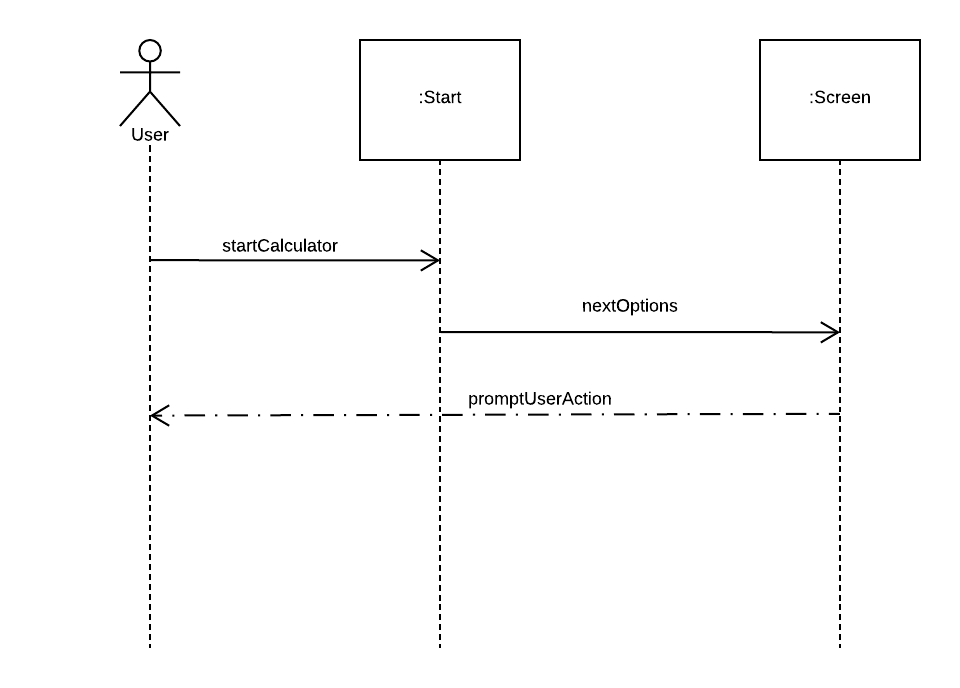
\includegraphics[width=80mm, height=50mm]{UseCase1.png}}
    \caption{UC001 Start Calculator}
    \label{fig:UC001 Start Calculator}
\end{figure}

\subsection{Use Case 2 - Enter a number(UC002)}
\quad The user enters the random number that will be used for the calculations. The calculator application will accept the input and display options on screen for user to proceed further.
\begin{figure}[!h]
    \centering
    \fbox{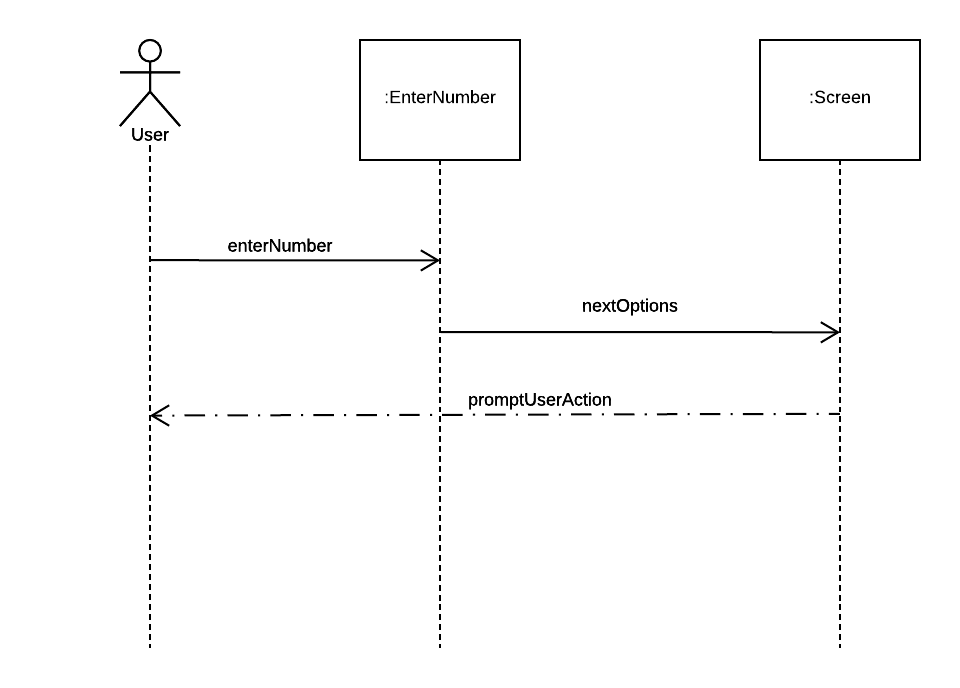
\includegraphics[width=80mm, height=50mm]{UseCase2.png}}
    \caption{UC002 Enter Number}
    \label{fig:UC002 Enter Number}
\end{figure}

\subsection{Use Case 3 - Choose type of Operation(UC003)}
\quad The user selects one of the options which is read by the calculator and starts processing the request or prompts user with messages if any other inputs are needed.\\\\
\begin{figure}[h]
    \centering
    \fbox{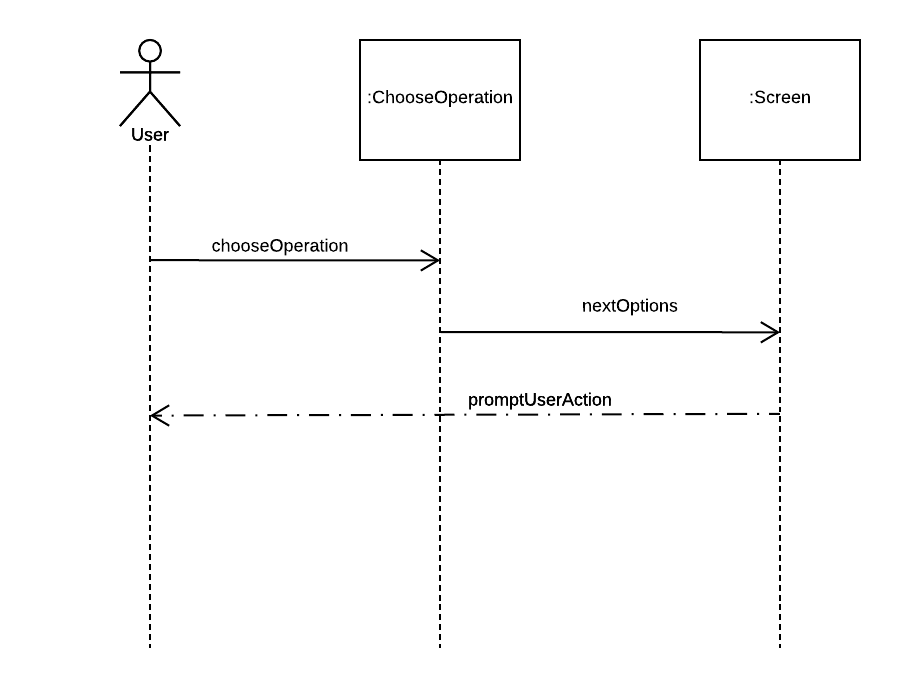
\includegraphics[width=100mm, height=80mm]{UseCase3.png}}
    \caption{UC003 Choose Type of Operation}
    \label{fig:UC003 Choose Type of Operation}
\end{figure}

\subsection{Use Case 4 - Perform Calculation(UC004)}
\quad The request opted from the user is picked up for processing and the calculator invokes relevant operation to process the data.
\begin{figure}[h]
    \centering
    \fbox{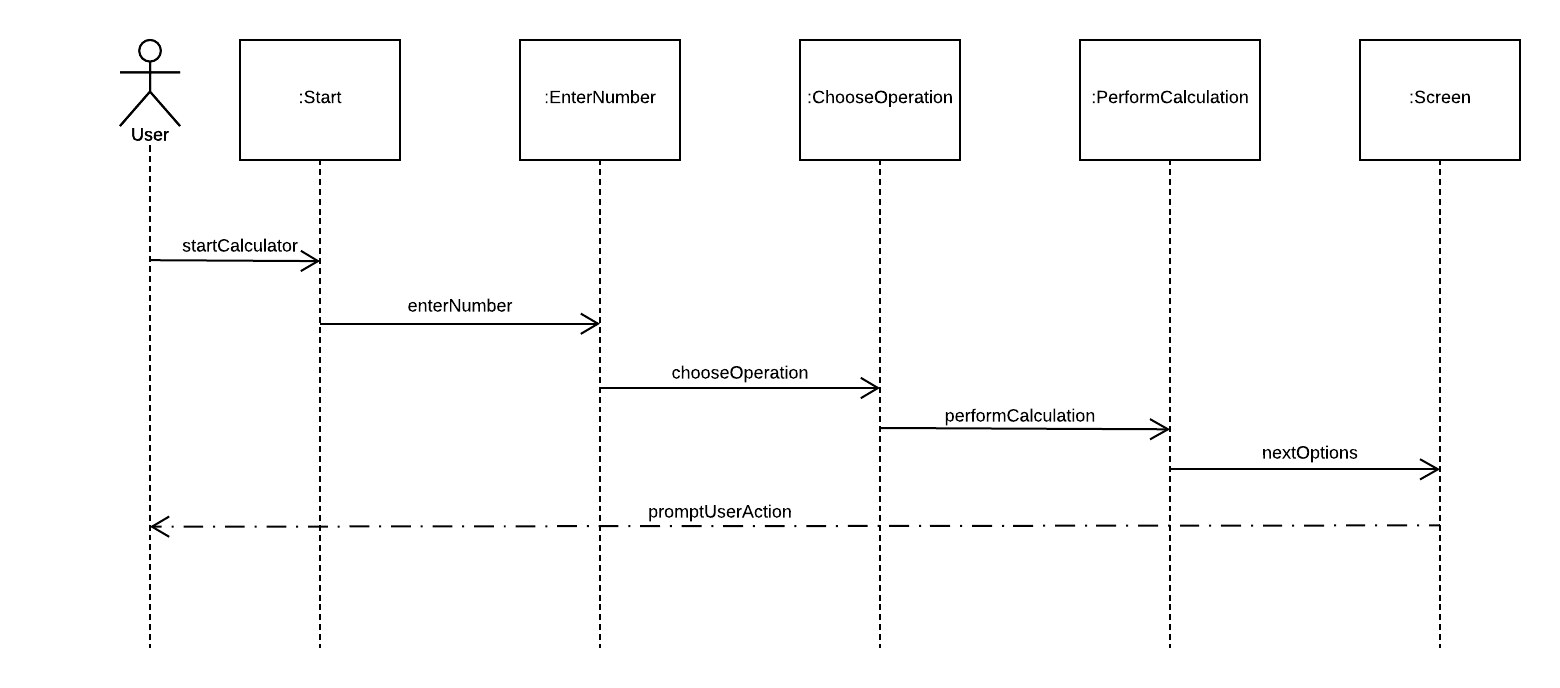
\includegraphics[width=140mm, height=80mm]{UseCase4.png}}
    \caption{UC004 Perform Calculation}
    \label{fig:UC004 Perform Calculation}
\end{figure}

\subsection{Use Case 5 - Generate Champernowne Constant}
\quad This is an extension of Perform Calculation which is invoked when the user selects one of the options to generate the Champernowne Constant.\\\\
\begin{figure}[h]
    \centering
    \fbox{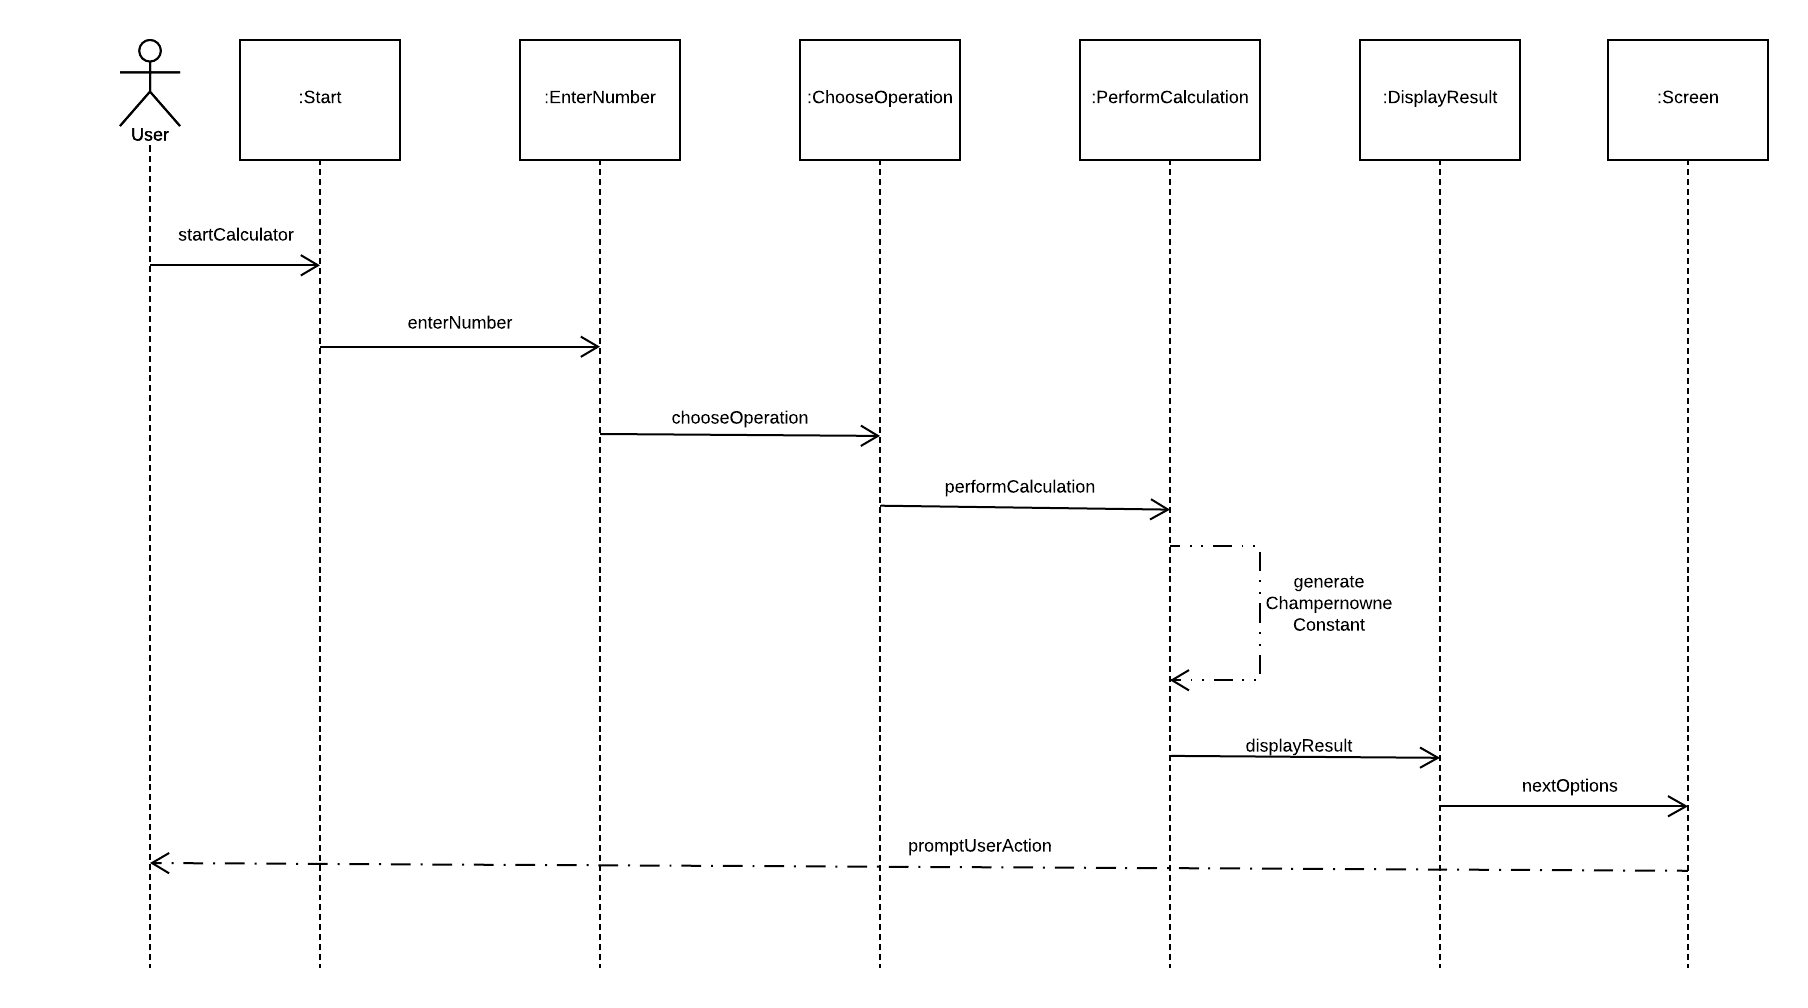
\includegraphics[width=160mm, height=80mm]{UseCase5.png}}
    \caption{UC005 Generate Champernowne Constant}
    \label{fig:UC005 Generate Champernowne Constant}
\end{figure}

\subsection{Use Case 6 - Display Result(UC006)}
\quad The results of the calculations performed based on user's choice are streamed to the console to be displayed to the user.
\begin{figure}[h]
    \centering
    \fbox{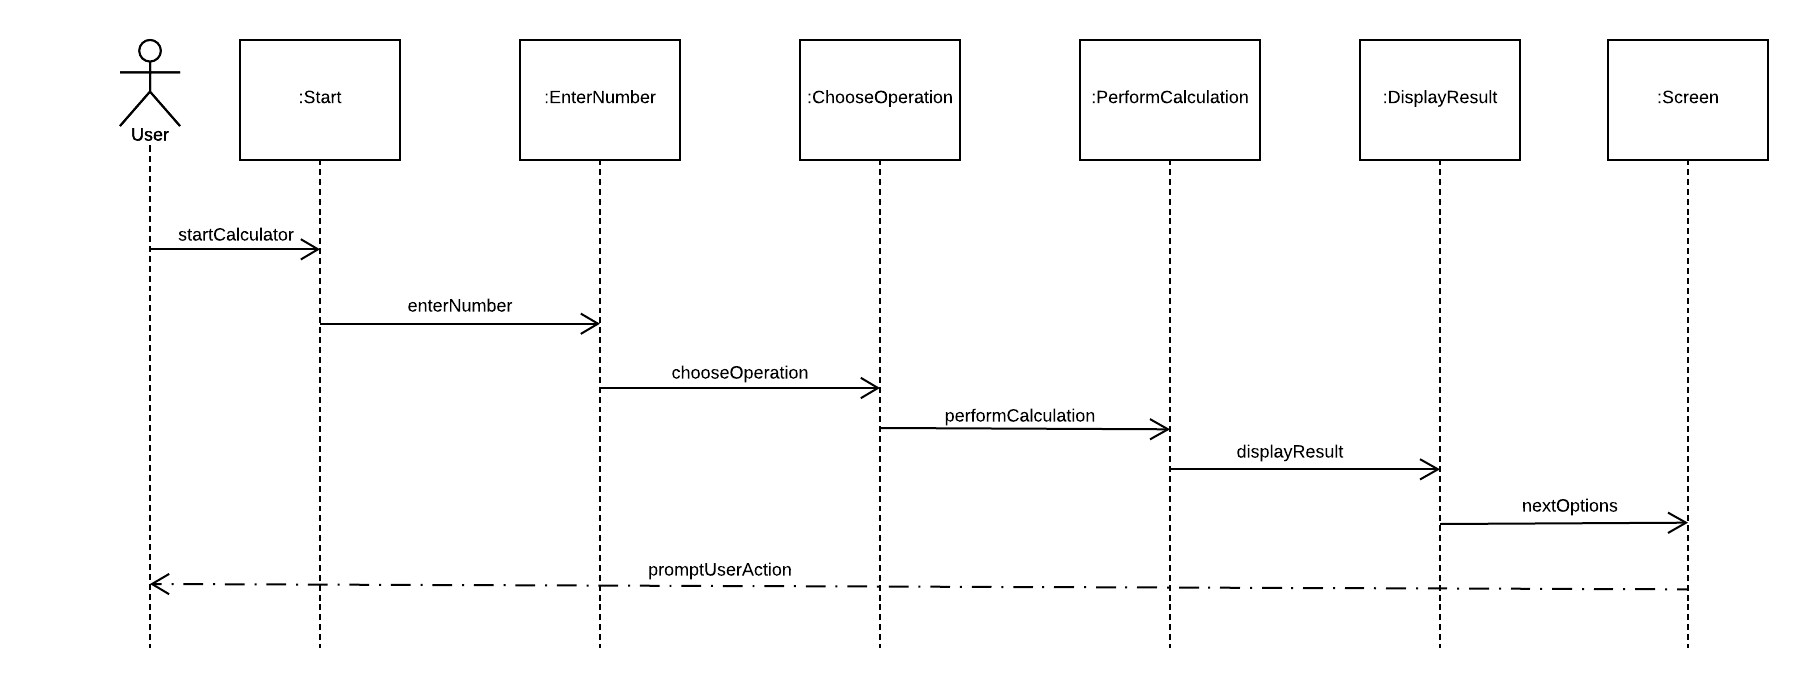
\includegraphics[width=160mm, height=80mm]{UseCase6.png}}
    \caption{UC006 Display Result}
    \label{fig:UC006 Display Result}
\end{figure}


\chapter{User stories and Acceptance Test cases}
\section{User stories and Acceptance Test cases}
The following table describes the list of user stories and acceptance test cases for every user story.
\\\\
\begin{tabular}{|p{3cm}|p{12cm}|}
\hline
     \textbf{US001} &  As a user, I want to find the position of a given number in the sequence of positive integers to calculate the total number of digits between 0 and the given number.\\\hline
     \textbf{Constraint} &  \textbf{1. } The input number cannot be a decimal or a negative number as the champernowne constant is a series of positive integers at base 10. \newline \textbf{2. } The number entered should always be numeric.\\\hline
     \textbf{Priority} & 5 \\\hline
     \textbf{Estimate} & 1 \\\hline
     \multirow{2}{3cm}{\textbf{Acceptance Test cases}} & \textbf{TC001} - Start the calculator application. Enter a random positive integer number as 100. Select "Find Position in Champernowne Constant" from the options menu. \newline \textbf{Output} - The position of number 100 in Champernowne Constant(C10) is 190.\\\cline{2-2}
     & \textbf{TC002} - Start the calculator application. Enter a random String as "abc". \newline \textbf{Output} - Please enter a valid positive integer number.\\\cline{2-2}
     & \textbf{TC003} - Start the calculator application. Enter a random positive decimal number. Select "Find Position in Champernowne Constant" from the options menu. \newline \textbf{Output} - Please enter a valid positive integer number.\\\hline
\end{tabular}
\\\\\\
\begin{tabular}{|p{3cm}|p{12cm}|}
\hline
     \textbf{US002} &  As a user, I want to save the random number entered by user and find its square value to display a message "The square of X is Y".\\\hline
     \textbf{Constraint} &  \textbf{1. } The number entered to calculate the square should always be numeric.\\\hline
     \textbf{Priority} & 4 \\\hline
     \textbf{Estimate} & 2 \\\hline
     \multirow{2}{3cm}{\textbf{Acceptance Test cases}} & \textbf{TC004} - Start the calculator application. Enter a random positive integer number as 3. Select "Save the number". Select "Find the square of the number". \newline \textbf{Output} - "The square of \textbf{3} is \textbf{9}"\\\cline{2-2}
     & \textbf{TC005} - Start the calculator application. Enter a random positive decimal number. Select "Find Position in Champernowne Constant" from the options menu. \newline \textbf{Output} - Please enter a valid positive integer number.\\\hline
\end{tabular}
\\\\\\\\
\\
\begin{tabular}{|p{3cm}|p{12cm}|}
\hline
     \textbf{US003} &  As a user, I want to calculate the Champernowne constant to generate the sequence of incremental positive numbers.\\\hline
     \textbf{Constraint} &  \textbf{1. } The input number cannot be a decimal or a negative number as the champernowne constant is a series of positive integers at base 10. \newline \textbf{2. } The number entered should always be numeric.\\\hline
     \textbf{Priority} & 3 \\\hline
     \textbf{Estimate} & 4 \\\hline
     \multirow{2}{3cm}{\textbf{Acceptance Test cases}} & \textbf{TC006} - Start the calculator application. Enter a random positive integer number as 12. Select "Generate Base 10 Champernowne Constant". \newline \textbf{Output} - The calculator application should display the message "The Base 10 Champernowne constant of length \textbf{12} digits is \textbf{0.123456789101}.\\\cline{2-2}
     & \textbf{TC007} - Start the calculator application. Enter a random positive decimal number. Select "Find Position in Champernowne Constant" from the options menu. \newline \textbf{Output} - Please enter a valid positive integer number.\\\hline
\end{tabular}
\\\\\\\\
\begin{tabular}{|p{3cm}|p{12cm}|}
\hline
     \textbf{US004} &  As a user, I want to generate random binary digits to use the random sequence to enable/disable relay switches.\\\hline
     \textbf{Constraint} &  \textbf{1. } The input number cannot be a decimal or a negative number as the champernowne constant is a series of binary digits at base 2. \newline \textbf{2. } The number entered should always be numeric.\\\hline
     \textbf{Priority} & 2 \\\hline
     \textbf{Estimate} & 8 \\\hline
     \multirow{2}{3cm}{\textbf{Acceptance Test cases}} & \textbf{TC008} - Start the calculator application. Enter a random positive integer number. Select "Generate Binary Champernowne constant". \newline \textbf{Output} - The Base 2 Champernowne constant of length \textbf{12} digits is \textbf{0.110111001011}\\\cline{2-2}
     & \textbf{TC009} - Start the calculator application. Enter a random positive decimal number. Select "Find Position in Champernowne Constant" from the options menu. \newline \textbf{Output} - Please enter a valid positive integer number.\\\hline
\end{tabular}
\\\\\\\\
\begin{tabular}{|p{3cm}|p{12cm}|}
\hline
     \textbf{US005} &  As a user, I want to find the positions of two different numbers in a sequence of positive integers to identify the number of digits between the two numbers.\\\hline
     \textbf{Constraint} &  \textbf{1. } The input number cannot be a decimal or a negative number as the champernowne constant is a series of positive integers at base 10. \newline \textbf{2. } The number entered should always be numeric.\\\hline
     \textbf{Priority} & 1 \\\hline
     \textbf{Estimate} & 16 \\\hline
     \multirow{2}{3cm}{\textbf{Acceptance Test cases}} & \textbf{TC010} - Start the calculator application. Enter a random positive integer number 10. Select "Find the position of the Number in Champernowne Constant". Select "Save the Number". Select "Find the square of a Number". Select "Find the position of the number in Champernowne Constant". Select "Previous Number". Select "Subtraction" between "Previous result" and  "Saved Number". \newline \textbf{Output} - The difference of \textbf{190} and \textbf{10} is \textbf{180}. \newline \textbf{Note}: 190 is the starting position of number 100(Square of 10 in this case) and 10 is the starting position of 10  \\\cline{2-2}
     & \textbf{TC011} - Start the calculator application. Enter a random positive decimal number. Select "Find Position in Champernowne Constant" from the options menu. \newline \textbf{Output} - Please enter a valid positive integer number.\\\hline
\end{tabular} 

\chapter {Backward Traceability Matrix}

\begin{longtable}{|p{1.5cm}|p{3cm}|p{2cm}|p{4cm}|}

    \hline
    User Stories & Use Cases & Persona & Requirements / Interview Questions \\\hline
    US001 & UC001, UC002, UC003, UC004, UC006 & X & 1,2,14\\\hline
    US002 & UC001, UC002, UC003, UC004, UC006 &NA &NA\\\hline
    US003 & UC001, UC002, UC003, UC004, UC005, UC006 & X & 14\\\hline
    US004 & UC001, UC002, UC003, UC004, UC005, UC006 & X & 10\\\hline
    US005 & UC001, UC002, UC003, UC004, UC005, UC006 & X & 1,2,14\\\hline
\caption{Table for Backward Traceability Matrix}
\label{table:1}
\end{longtable}
{*Refer Figure 6.1 for the User Stories and Figure 5.1 for the Use Case Diagram.}

\\
\chapter{Eternity:Numbers Calculator}

\section{Generic Guidelines}

\quad To launch the Eternity:Numbers calculator application, please follow the below steps - 

\begin{itemize}
    \item Download the source code from the git repository \newline \underline{https://github.com/NikithaBangera/SOEN6481Project}
    \item Open Eclipse,
    \item Select File, and choose Open Project from FileSystem,
    \item Browse to the location where you downloaded the .zip file from the git repository,
    \item Select the project folder and click Ok,
    \item Open the EternityNumber.java file,
    \item Right click anywhere in the window and Select Run As - Java Application.
\end{itemize} 

\section{Guidelines for User Stories}

\subsection{User Story 1(US001)}
\begin{itemize}
    \item The calculator application prompts to enter a number,
    \item Enter a number 100 and hit Enter,
    \item Now enter 8, to select Option "8.Find the position in Champernowne Constant(C10)" and hit Enter,
    \item The calculator application will display a message "The position of 100 in Champernowne constant(C10) is 190".
\end{itemize}

\subsection{User Story 2(US002)}
\begin{itemize}
    \item The calculator application prompts to enter a number.
    \item Enter a number 10 and hit Enter.
    \item Now enter 6, to select Option "6. Square of a number" and hit Enter.
    \item The calculator application will display a message "The square of 10 is 100".
\end{itemize}

\subsection{User Story 3(US003)}
\begin{itemize}
    \item The calculator application prompts to enter a number.
    \item Enter a number 12 and hit Enter.
    \item Now enter 10, to select Option "10. Generate base 10 Champernowne Constant(C10)" and hit Enter.
    \item The calculator application will display a message "The base 10 Champernowne constant of length 12 digits is 0.123456789101".
\end{itemize}

\subsection{User Story 4(US004)}
\begin{itemize}
    \item The calculator application prompts to enter a number.
    \item Enter a number 12 and hit Enter.
    \item Now enter 9, to select Option "9. Generate a binary Champernowne constant(C2)" and hit Enter.
    \item The calculator application will display a message "The base 2 Champernowne constant of length 12 digits is 0.110111001011".
\end{itemize}

\subsection{User Story 5(US005)}
\begin{itemize}
    \item The calculator application prompts to enter a number.
    \item Enter a number 10 and hit Enter.
    \item Now enter 8, to select Option "8. Find the position in Champernowne Constant(C10)" and hit Enter.
    \item The calculator application will display a message "The position of 10 in Champernowne constant(C10) is 10".
    \item Now enter 11, to select Option "11. Save the number" and hit Enter.
    \item The calculator application should display the message "Number 10 saved successfully.".
    \item Now enter 6, to select Option "6. Square of a number" and hit Enter.
    \item The calculator application will display options to select which number to choose to calculate the square value.
    \item Now enter 1, to select Option "1.Saved Number" and hit Enter.
    \item The calculator application should display the message "The square of 10 is 100.0".
    \item Now enter 8, to select Option "8. Find the position in Champernowne Constant(C10)" and hit Enter.
    \item The calculator application will display options to select which number to choose to proceed further.
    \item Now enter 2, to select Option "2.Previous Result" and hit Enter.
   \item The calculator application should display the message "The position of 100 in Champernowne constant(C10) is 190".
   \item Now enter 2, to select option "2. Subtraction" and hit Enter.
   \item The calculator application will display options to select which number to choose as first number for subtraction.
   \item Now enter 2, to select Option "2.Previous Result" and hit Enter.
    \item The calculator application will display options to select which number to choose as Second number for subtraction.
    \item Now enter 1, to select Option "1.Saved Number" and hit Enter.
    \item The calculator application should display a message "The difference of 190 and 10 is 180".
\end{itemize}

\chapter{Version Control Repository}
The link for my Github Repository is given below:\\
\url{https://github.com/NikithaBangera/SOEN6481Project}

\begin{thebibliography}{9}
    \bibitem {Wikipedia}
    \texttt{https://en.wikipedia.org/wiki/Champernowne{\_}constant}
    \bibitem {Wolfram}
    \texttt{http://mathworld.wolfram.com/ChampernowneConstant.html}
    \bibitem{wikia}
    \texttt{https://googology.wikia.org/wiki/Champernowne{\_}constant{\_}continued{\_}fraction}
    \bibitem {FSE}
    \texttt{http://fse.studenttheses.ub.rug.nl/}
    \bibitem {Online Encyclopedia Champernowne constant base 10}
    \texttt{https://oeis.org/A065649}
    \bibitem {An Interesting property of Champernowne's number}
    \texttt{https://www.kanonical.io/an{\_}interesting{\_}property{\_}of{\_}champernownes{\_}number/}
\end{thebibliography}
\end{document}
